\documentclass{article}
\usepackage[utf8]{inputenc}
\usepackage[english]{babel}
\usepackage{graphicx}

\usepackage{xcolor}

\title{Report}
\author{Egirin Gega \&  Samuli Romo}

\begin{document}
  \maketitle

  \newpage
  \tableofcontents
  \newpage
  \listoffigures
  \newpage
  \listoftables

  \newpage
  \section{Convolutional Neural Network}
  A Convolutional Neural Network also known as a CNN or COMV NET is an artificial neural network that is so far been most popularly used for analyzing images. Although image analysis has been the most widespread use of CNN's they can also be used for other data analysis or classification problems as well most generally.
  \subsection{How does it Work}
    \paragraph{}
    We can think of a CNN as an artificial neural network that has some type of specialization for being able to pick out or detect patterns and make sense of them. This pattern detection is what makes CNN so useful for image analysis so if a CNN is just some form  neural network what differentiates it from just a standard multi-layer perceptron or MLP well  these layers are precisely what makes a CNN a CNN.
    \begin{figure}[h!]
      \begin{center}
        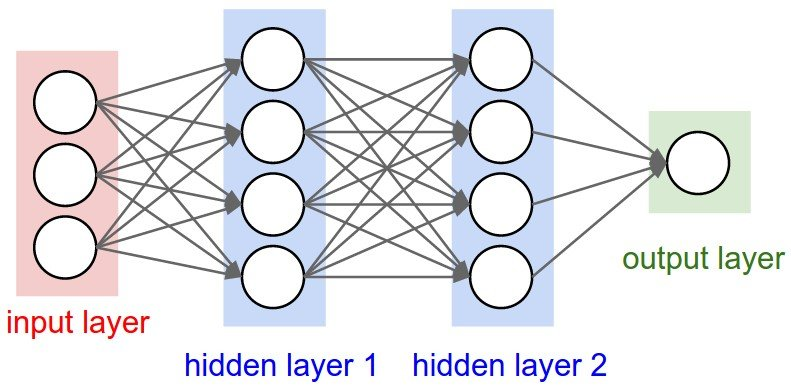
\includegraphics[width=0.7\linewidth]{img/Visualization-of-a-traditional-fully-connected-neural-network-Stanford-University.png}
        \caption{Simple Representation.}
        \label{fig:snn}
      \end{center}
    \end{figure}
    \paragraph{}
    CNN's can and usually do have other non convolutional layers as well but the basis of a CNN is the convolutional layers all right so what do these convolutional layers do just like any other layer a convolutional layer receives input then transforms the input in some way and then outputs the transform input to the next layer with a convolutional layer this transformation is a convolution operation.
    \paragraph{}
    Most generally we can think of a CNN as an artificial neural network that has some type of specialization for being able to pick out or detect patterns and make sense of them. This pattern detection is what makes CNN so useful for image analysis.So if a CNN is just some form of an artificial neural network what differentiates it from just a standard multi-layer perceptron or MLP?
    \paragraph{} 
    Well a CNN has hidden layers called convolutional layers and these layers are precisely what makes a CNN well a CNN. Now CNN's can and usually do have other non convolutional layers as well but the basis of a CNN is the convolutional layers.
    \vspace{20mm}
  \section{Recurrent Neural Network}
  Recurrent neural networks are learning model with a simple structure  and a built-in feedback loop, allowing it  to act as a forecasting engine. 
  Recurrent neural networks, or RNNs, have  a long history, but their recent popularity  is mostly due to the works of Juergen Schmidhuber,  Sepp Hochreiter, and Alex Graves. Their applications  are extremely versatile, ranging from speech  recognition to driverless cars.
  \subsection{How does it Work}
    \paragraph{}
    All the nets we’ve seen up to this point  have been feedforward neural networks. In  a feedforward neural network, signals flow  in only one direction from input to output,  one layer at a time. In a recurrent net, the  output of a layer is added to the next input  and fed back into the same layer, which is  typically the only layer in the entire network.  You can think of this process as a passage  through time – shown here are 4 such time  steps. At t = 1, the net takes the output  of time t = 0 and sends it back into the net  along with the next input. The net repeats  this for t = 2, t = 3, and so on.  Unlike feedforward nets, a recurrent net can  receive a sequence of values as input, and  it can also produce a sequence of values as  output. The ability to operate with sequences  opens up these nets to a wide variety of applications.

    \begin{figure}[h!]
      \begin{center}
        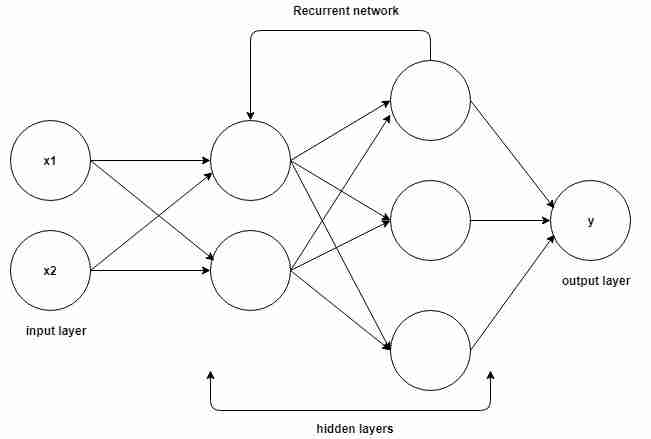
\includegraphics[width=0.5\linewidth]{img/Recurrent.jpeg}
        \caption{Recurrent Neural Network.}
        \label{fig:snn}
      \end{center}
    \end{figure}
    
    \paragraph{}
    Here are a few examples. When the input is  singular and the output is a sequence, a potential  application is image captioning. A sequence  of inputs with a single output can be used  for document classification. When both the  input and output are sequences, these nets  can classify videos frame by frame. If a time  delay is introduced, the net can statistically  forecast the demand in supply chain planning.  Have you ever used an RNN for one of these  applications? If so, please comment and share  your experiences.  Like we’ve seen with previous deep learning  models, by stacking RNNs on top of each other,  you can form a net capable of more complex  output than a single RNN working alone.
    \paragraph{}
    Typically, an RNN is an extremely difficult  net to train. Since these nets use backpropagation,  we once again run into the problem of the  vanishing gradient. Unfortunately, the vanishing  gradient is exponentially worse for an RNN.  The reason for this is that each time step  is the equivalent of an entire layer in a  feedforward network. So training an RNN for  100 time steps is like training a 100-layer  feedforward net – this leads to exponentially  small gradients and a decay of information  through time.  There are several ways to address this problem  - the most popular of which is gating. Gating  is a technique that helps the net decide when  to forget the current input, and when to remember  it for future time steps. The most popular  gating types today are GRU and LSTM. Besides  gating, there are also a few other techniques  like gradient clipping, steeper gates, and  better optimizers.
    \paragraph{}
    When it comes to training a recurrent net,  GPUs are an obvious choice over an ordinary  CPU. This was validated by a research team  at Indico, which uses these nets on text processing  tasks like sentiment analysis and helpfulness  extraction. The team found that GPUs were  able to train the nets 250 times faster! That’s  the difference between one day of training,  and over eight months!  So under what circumstances would you use  a recurrent net over a feedforward net? We  know that a feedforward net outputs one value,  which in many cases was a class or a prediction.  A recurrent net is suited for time series  data, where an output can be the next value  in a sequence, or the next several values.  So the answer depends on whether the application  calls for classification, regression, or forecasting.

    \newpage
    \section{CNN vs RNN Comparison in time series applications}
    Although CNNs and RNNs are both neural networks and can process some of the same input types, they are structured differently and applied for different purposes.

\end{document}